\documentclass[11pt]{report}
\usepackage[utf8]{inputenc} 
\usepackage{graphicx}

\begin{document}

\title{Simple Character Driver - SCD}
\author{Nemanja Hiršl}

\maketitle
\tableofcontents
\newpage

\section{Requirements}
To implement character device for Debian, which will be able to work as exchange point between two user-space processes (e.g. stream BLOB file between them).\\
Requirements:\\
Programing Languages: C (mandatory for driver), C/C++ (for user space applications)\\
OS: Debian (openWRT) \\
Platform: x86,x64 \\
Features to be implemented:
\begin{enumerate}
\item Character device to be created (file of device to be created when driver is being registered in system (if it doesn’t exist))
\item Main file operations to e implemented
\begin{itemize}
\item Read (to read data from device in user-space).Data should be returned to user-space application when it requests it using “read” function.
\item Write (to write data to device from user-space). Data acquired from one user-space process should go to another one. Driver should be able to signalize that data is ready (via response in “poll” call).
\item Poll (to wait for data on device in user-space). User-space application should be able to  hang in poll function and get correct response from this function when data in driver is ready (as it is in man, if applicable)
\item Ioctl (to configure device from user-space). Configuration of device could be needed (any needed user-space application parameters or runtime options should be sent to driver via this call)
\end{itemize}
\item Logging (detailed and basic) to be implemented. Should be configurable
\end{enumerate}

\section{Introduction}
Simple Character Driver: SCD is character driver which acts on memory area as it is a hardware device. Per requirements it is designed to work as exchange point between two user space processes. It is similar to pipe and is implemented by using circular buffer for storing data. Multiple readers or writers are supported, but each read or write will alter the internal buffer and the change will affect others. Example is one writer and two readers: Data is not preserved between readers and each might end up getting just the portion of what writer has written to device. It is up to user space programs to handle such situations. In other words: One process reads what another process writes. If multiple processes read the same device, they contend for data. SCD implements mutual exclusion mechanism for synchronizing concurrent access to the internal buffer. Opening a device will reset internal buffer, thus all parties involved in data exchange should open the device prior to any attempt to read or write. 

\section{Dependencies}
Not all dependencies are required for successful build of SCD, but they are highly recommended.
\begin{itemize}
\item Environment for kernel module building (out of scope of this document)
\item make. Needed for building the project.
\item bash. Needed for running install scripts.
\item indent. Used for formating C code.
\item astyle. Used for formating C++ code.
\item gtest. All tests are written with gtest lib. Makefiles assume that libgtest and libgtest\_main libraries can be found on standard libs locations.
\item latex, pdflatex. Needed for building documentation.
\item openssl. Needed for verification of transfered data.
\end{itemize}

\section{Build and install instructions}
Makefiles are used for building all parts of the SCD.
\begin{enumerate}
\item make
\item sudo make install
\end{enumerate}
The install step will just enter the SimpleCharacterDriver/scripts folder and execute \emph{scd\_load.sh}. If there is need for setting up Major num at load time, either Makefile should be updated or one should manually invoke \emph{scd\_load.sh} with appropriate parameters. Detailed explanation of the script follows.
Verify the module has been loaded successfully:
\begin{verbatim}
lsmod | grep scd
ls -l /dev/scd
tail -f /var/log/syslog
\end{verbatim}
The last item is optional and would show messages module has written to the log (truncated):
\begin{verbatim}
scd_init_module. Major: 0, minor: 0
scd_init_module. init device: 0
\end{verbatim}
Or on exit:
\begin{verbatim}
scd_exit_module. Major: 249, minor: 0
\end{verbatim}

Make will build tests, documents and all additional programs. After successful building, test executables will be available in Tests folder, this document as pdf generated from latex and executables for all programs (currently only 1) in appropriate directory.

\section{SCD internals}
SCD code is located in SimpleCharacterDriver folder and is separated in two files: \emph{scd.h} and \emph{scd.c}. \emph{scd.h} contains defines and \emph{scd.c} contains code for kernel module. Scripts for installing and uninstalling are provided and can be found in scripts subfolder.
\subsection{Kernel module}
Kernel module implements:
\begin{verbatim}
/* The file operations for the device. */
static struct file_operations scd_pipe_fops = {
	.owner = THIS_MODULE,
	.read = scd_read,
	.write = scd_write,
	.poll = scd_poll,
	.unlocked_ioctl = scd_unlocked_ioctl,
	.open = scd_open,
	.release = scd_release,
	.llseek = no_llseek,
};
\end{verbatim}
At load time, module supports setting Major and Minor numbers:
\begin{verbatim}
	/* Module parameters assignable at load time. */
	module_param(scd_major, int, S_IRUGO);
	module_param(scd_minor, int, S_IRUGO);
\end{verbatim}

\subsubsection{Memory handling}
Device is represented as circular buffer. The size of the buffer is 32K by default, but it can be changed from the user space programs.
\begin{verbatim}
	char *begin, *end;	/* begin of buffer, end of buffer */
	char *read, *write;	/* where to read, where to write */
\end{verbatim}
are used to handle reading and writing data from and to circular buffer.

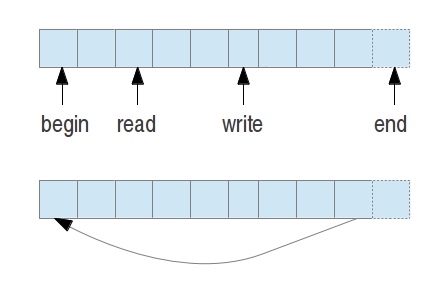
\includegraphics[scale=0.5]{Buffer}

Whenever \emph{read == write}, we've read everything and there is no new data for reading. Writing can occur whenever there is free space in the buffer. Buffer is considered full when \emph{write} is \emph{just} behind the \emph{read}
\begin{enumerate}
\item Read and Write are on the same position, nothing to read: Available space for writing is buffersize - 1.
\item Read is ahead of Write. Available space is just up to the read pointer.
\item Write is ahead of Read. Available space is everything except non read part.
\end{enumerate}

\subsection{Scripts}
Two scripts for loading, unloading, creating and deletion of the kernel module and device are provided: \emph{scd\_load.sh} and \emph{scd\_unload.sh}. They are allowing users to provide their own Major number for driver at load time and control how device is created. User must be root in order to execute these scripts. \emph{scd\_load.sh} has some basic input validation and usage is per help: 
\begin{verbatim}
		Usage: scd_load.sh [-h] [-M MajorNum] [-m MinorNum]
		Will load a module with predefined MajorNum and MinorNum.
       		-h          Display this help and exit
       		-M MajorNum Set desired MajorNum.
       		-m MinorNum Set desired MinorNum.
\end{verbatim}
\emph{scd\_unload.sh} is minimal and it will just unload the module (rmmod) and delete device.
TODO section proposes some improvements for scripts.

\section{Test plan}
\subsection {Driver tests}
This group of tests should cover basic (unit) functionality of the driver. It should explicitly test all of supported functions. Some of these tests are automated and can be found in Tests/Driver folder. These are implemented by using gtest as external library. 

\subsection {System tests}
System tests are those related to: loading, unloading, creating and deletion of module and device. There are two bash scripts provided for this purpose and these should be thoroughly tested. Cases when Major number is provided and (in)valid must be covered. Verification of (un)successful loading and unloading must be implemented. Ideally, these tests should be automated. 

\subsection {Integration tests}
Integration tests are covering complex environment where two user space programs exchange data through the device. Some tests are automated and can be found in Tests/Driver folder.These are implemented by using gtest as external library.

\subsection {Performance tests}
Depending of the driver's buffer size and size of the data which is transfered, performance results may vary. Collecting and examining such data might be valuable for future improvements in the driver. None of these tests are currently covered.  

\subsection {Automated test results}
All automated tests are passing.

\subsection{Programs}
Additional program(s) are just small examples how streaming might look like by using scd device (proof of concept). They are tests which require user's interaction. Program \emph{writer} will block and wait for a file to appear in \emph{./} folder. This file will be copied to scd device. It could be used to test big data transfer.
Example:
\begin{enumerate}
\item Open two consoles. Navigate to \emph{Home} from one and \emph{Programs/Writer} from the other console.
\item Start listening on device in \emph{Home}, e.g: \begin{verbatim} cat /dev/scd > myfile.dat \end{verbatim}
\item Start \emph{writer} program in the other console. It will block waiting for new file to appear in the current folder.
\item Put big file \emph{myOrigFile} in the \emph{Writer} folder. The transfer will start and the logs will indicate successful transfer.
\item Verify transfer:
\begin{enumerate}
\item In \emph{Writer} folder do \begin{verbatim} openssl sha1 myOrigFile \end{verbatim}
\item In \emph{Home} folder do \begin{verbatim} openssl sha1 myfile.dat \end{verbatim}
\item Verify the numbers are the same.
\end{enumerate}
\end{enumerate}

\section{TODO}
There are things which should be improved and/or finished. This is current list:
\begin{enumerate}
\item SCD
\begin{enumerate}
\item Consider better memory handling for circular buffer. Implement memory reallocation on ioctl (scd\_unlocked\_ioctl)
\item Implement capabilities.
\item Support number (\textgreater 1) of devices.
\end{enumerate}
\item Scripts. Make scripts more robust and provide init script for loading at startup (systemd). Handle multiple devices.
\item Tests.
\begin{enumerate}
\item Create and document detailed test cases
\item Consider expanding and improving Driver tests
\item Automate test cases for loading/unloading driver (provided vs dynamic Majors)
\item Verify successful module registration
\item Consider automatic test results inclusion in documentation
\end{enumerate}
\item Programs. Make example programs more robust and bullet prof. As of today, they are proof of concept and should handle better all flow paths. The best solution would be to make a c++ wrapper class which handles all operations for SimpleExchangeDriver and which could be used as an API for accessing the device.
\end{enumerate}

\end{document}
